\subsection*{Teil B: Projekt - Schulpavilion planen (70 Minuten)}

\textbf{Aufgabe:} Eure Schule möchte einen neuen Pavilion für Pausenaktivitäten bauen. Ihr seid die Planungsgruppe!

\begin{enumerate}[label=\arabic*.,resume]

    \item \textbf{Grundriss planen (Dreiecke und Vierecke) - 25 Minuten}

    Der Pavilion soll einen achteckigen Grundriss haben, der aus einem Rechteck (12 m × 8 m) und vier angebauten gleichschenkligen Dreiecken besteht.

    \begin{enumerate}[label=\alph*)]
        \item Zeichne den Grundriss (Maßstab 1:200):

        \vspace{6cm}

        \item Prüfe, ob aus den Maßen 3 m, 3 m und 4 m ein Dreieck konstruiert werden kann:

        \vspace{2cm}

        \item Berechne die Fläche des Rechtecks:

        \vspace{1.5cm}

        \item Berechne die Fläche eines Dreiecks (Basis 4 m, Höhe 2,5 m):

        \vspace{1.5cm}

        \item Gesamtgrundfläche des Pavilions:

        \vspace{1.5cm}

    \end{enumerate}

    \item \textbf{Kostenplanung (Terme und Gleichungen) - 20 Minuten}

    Die Baukosten setzen sich zusammen aus:
    - Fixkosten (Planung, Genehmigungen): 8.000 €
    - Variable Kosten pro m² Grundfläche: 350 €

    \begin{enumerate}[label=\alph*)]
        \item Stelle die Kostenfunktion auf: $K(A) = $ \underline{\hspace{6cm}}

        \item Berechne die Gesamtkosten für euren Pavilion:

        \vspace{2cm}

        \item Das Budget beträgt 25.000 €. Wie groß darf die maximale Grundfläche sein?

        Gleichung aufstellen und lösen:

        \vspace{3cm}

        \item Vereinfache den Term: $5(2x + 3) - 3(x - 1) = $ \underline{\hspace{6cm}}

        \vspace{1cm}

    \end{enumerate}

    \item \textbf{Regenwasser-Sammlung (Funktionen) - 15 Minuten}

    Auf dem Dach soll Regenwasser gesammelt werden. Die Dachfläche beträgt 150 m².

    Pro mm Niederschlag sammeln sich 150 Liter Wasser. Der Tank fasst 5000 Liter und ist zu Beginn leer.

    \begin{enumerate}[label=\alph*)]
        \item Funktionsgleichung: $V(n) = $ \underline{\hspace{6cm}} (V in Litern, n in mm Niederschlag)

        \item Zeichne die Funktion bis der Tank voll ist:

        \begin{center}
            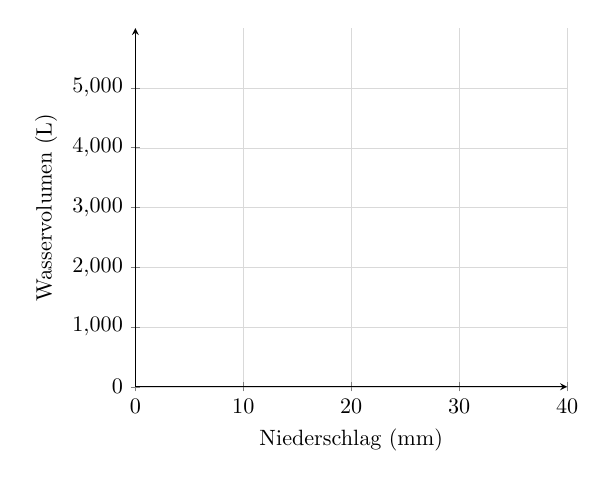
\begin{tikzpicture}[scale=0.8]
                \begin{axis}[
                    axis lines = left,
                    xlabel = {Niederschlag (mm)},
                    ylabel = {Wasservolumen (L)},
                    xmin=0, xmax=40,
                    ymin=0, ymax=6000,
                    xtick={0,10,20,30,40},
                    ytick={0,1000,2000,3000,4000,5000},
                    grid=major,
                    grid style={line width=0.1pt,draw=gray!30},
                ]
                \end{axis}
            \end{tikzpicture}
        \end{center}

        \item Nach wie viel mm Niederschlag ist der Tank voll?

        \vspace{2cm}

        \item Bei 15 mm Niederschlag, wie viel Wasser ist im Tank?

        \vspace{1.5cm}

    \end{enumerate}

    \item \textbf{Materialberechnung (Raumgeometrie) - 10 Minuten}

    Für das Dach werden zylindrische Stützsäulen benötigt:
    - Durchmesser: 30 cm  
    - Höhe: 3,5 m
    - Anzahl: 6 Stück

    \begin{enumerate}[label=\alph*)]
        \item Volumen einer Säule:

        \vspace{2cm}

        \item Gesamtvolumen aller Säulen in m³:

        \vspace{1.5cm}

        \item Die Säulen werden aus Beton gegossen. 1 m³ Beton kostet 120 €. Wie viel kosten alle Säulen?

        \vspace{2cm}

        \item Oberfläche einer Säule (ohne Boden und Deckel):

        \vspace{2cm}

    \end{enumerate}

\end{enumerate}